%% fcup-thesis.tex -- document template for PhD theses at FCUP
%%
%% Copyright (c) 2015 João Faria <joao.faria@astro.up.pt>
%%
%% This work may be distributed and/or modified under the conditions of
%% the LaTeX Project Public License, either version 1.3c of this license
%% or (at your option) any later version.
%% The latest version of this license is in
%%     http://www.latex-project.org/lppl.txt
%% and version 1.3c or later is part of all distributions of LaTeX
%% version 2005/12/01 or later.
%%
%% This work has the LPPL maintenance status "maintained".
%%
%% The Current Maintainer of this work is
%% João Faria <joao.faria@astro.up.pt>.
%%
%% This work consists of the files listed in the accompanying README.

%% SUMMARY OF FEATURES:
%%
%% All environments, commands, and options provided by the `ut-thesis'
%% class will be described below, at the point where they should appear
%% in the document.  See the file `ut-thesis.cls' for more details.
%%
%% To explicitly set the pagestyle of any blank page inserted with
%% \cleardoublepage, use one of \clearemptydoublepage,
%% \clearplaindoublepage, \clearthesisdoublepage, or
%% \clearstandarddoublepage (to use the style currently in effect).
%%
%% For single-spaced quotes or quotations, use the `longquote' and
%% `longquotation' environments.


%%%%%%%%%%%%         PREAMBLE         %%%%%%%%%%%%

%%  - Default settings format a final copy (single-sided, normal
%%    margins, one-and-a-half-spaced with single-spaced notes).
%%  - For a rough copy (double-sided, normal margins, double-spaced,
%%    with the word "DRAFT" printed at each corner of every page), use
%%    the `draft' option.
%%  - The default global line spacing can be changed with one of the
%%    options `singlespaced', `onehalfspaced', or `doublespaced'.
%%  - Footnotes and marginal notes are all single-spaced by default, but
%%    can be made to have the same spacing as the rest of the document
%%    by using the option `standardspacednotes'.
%%  - The size of the margins can be changed with one of the options:
%%     . `narrowmargins' (1 1/4" left, 3/4" others),
%%     . `normalmargins' (1 1/4" left, 1" others),
%%     . `widemargins' (1 1/4" all),
%%     . `extrawidemargins' (1 1/2" all).
%%  - The pagestyle of "cleared" pages (empty pages inserted in
%%    two-sided documents to put the next page on the right-hand side)
%%    can be set with one of the options `cleardoublepagestyleempty',
%%    `cleardoublepagestyleplain', or `cleardoublepagestylestandard'.
%%  - Any other standard option for the `report' document arclass can be
%%    used to override the default or draft settings (such as `10pt',
%%    `11pt', `12pt'), and standard LaTeX packages can be used to
%%    further customize the layout and/or formatting of the document.

%% *** Add any desired options. ***
%PDF
%\documentclass[a4paper,narrowmargins,12pt,oneside,draft,onehalfspaced,singlespacednotes]{fcup-thesis}
%\documentclass[a4paper,narrowmargins,12pt,oneside,onehalfspaced,singlespacednotes]{fcup-thesis}
%Print
%\documentclass[draft,a4paper,narrowmargins,12pt,twoside,openright,onehalfspaced,singlespacednotes]{fcup-thesis}
\documentclass[a4paper,narrowmargins,12pt,twoside,openright,onehalfspaced,singlespacednotes]{fcup-thesis}

%% *** Add \usepackage declarations here. ***
%% The standard packages `geometry' and `setspace' are already loaded by
%% `ut-thesis' -- see their documentation for details of the features
%% they provide.  In particular, you may use the \geometry command here
%% to adjust the margins if none of the ut-thesis options are suitable
%% (see the `geometry' package for details).  You may also use the
%% \setstretch command to set the line spacing to a value other than
%% single, one-and-a-half, or double spaced (see the `setspace' package
%% for details).
% Overfull statements
\pretolerance=150
\setlength{\emergencystretch}{3em}
% Overfull end
\usepackage[english]{babel}
\usepackage{lipsum}
\usepackage[utf8]{inputenc}


%%% Additional useful packages
%%% ----------------------------------------------------------------
\usepackage{array}
\usepackage{amsmath}  
\usepackage{amssymb}
\usepackage{amsfonts}
\DeclareFontFamily{OT1}{pzc}{}
\DeclareFontShape{OT1}{pzc}{m}{it}{<-> s * [0.900] pzcmi7t}{}
\DeclareMathAlphabet{\mathpzc}{OT1}{pzc}{m}{it}
\usepackage{amsthm}      
\usepackage[ruled,algochapter]{algorithm2e}
\usepackage{algorithmic}
\usepackage{bm}
\usepackage[mathscr]{euscript}
\usepackage{graphicx}       
\usepackage{psfrag}         
\usepackage{fancyvrb}    
\usepackage{float}
\usepackage{ltablex}
\usepackage[square,sort,comma,numbers]{natbib}        
\usepackage{bbding}         
\usepackage{dcolumn}        
\usepackage{booktabs} 
\usepackage{multirow}
\usepackage{paralist}     
\usepackage{ifdraft}  
\usepackage{indentfirst}    
\usepackage[nottoc,notlof,notlot]{tocbibind}
\usepackage{url}
\usepackage{tabularx}
\usepackage{subcaption}
\usepackage[unicode]{hyperref}
\usepackage{xcolor}

\hypersetup{pdftitle=LiDAR obstacle detection and avoidance, 
            pdfauthor=Alojz Gomola,
            colorlinks=false,
            urlcolor=blue,
            pdfstartview=FitH,
            pdfpagemode=UseOutlines,
            pdfnewwindow,
            breaklinks
          }
\usepackage{array}
\newcolumntype{L}[1]{>{\raggedright\let\newline\\\arraybackslash\hspace{0pt}}m{#1}}
\newcolumntype{C}[1]{>{\centering\let\newline\\\arraybackslash\hspace{0pt}}m{#1}}
\newcolumntype{R}[1]{>{\raggedleft\let\newline\\\arraybackslash\hspace{0pt}}m{#1}}         
\newcolumntype{B}{X}
\newcolumntype{S}[1]{>{\hsize=#1\textwidth}X}

\newcommand{\FIGDIR}{./Pics}    %%% directory containing figures
\newcommand{\twolinecellr}[2][r]{%
  \begin{tabular}[#1]{@{}r@{}}#2\end{tabular}}
\newcommand{\secState}[1]{
	\ifdraft{(#1) }{}
}
\theoremstyle{plain}
\newtheorem{theorem}{Theorem}
\newtheorem{lemma}[theorem]{Lemma}
\newtheorem{proposition}[theorem]{Proposition}

\theoremstyle{plain}
\newtheorem{definition}{Definition}
\newtheorem{problem}{Problem}
\newtheorem{example}{Example}
\newtheorem{assumption}{Assumption}

\theoremstyle{remark}
\newtheorem*{corollary}{Corollary}
\newtheorem*{note}{Note}




\newenvironment{dokaz}{
  \par\medskip\noindent
  \textit{Proof}.
}{
\newline
\rightline{\SquareCastShadowBottomRight}
}

\newenvironment{constraints}[1]{
  \par\medskip\noindent
  \textit{Constraints #1} \\
}{
\newline
\rightline{\SquareCastShadowBottomRight}
}


%\bibliographystyle{plainnat}     %% Author (year) style
\bibliographystyle{unsrt}        %% [number] style
\setcitestyle{square}

% Section  3.7 Challenge list
\newif\ifproblemchallenge   %# Build block for problem challenges
\problemchallengetrue       %# Show comments

\newcommand{\R}{\mathbb{R}}
\newcommand{\N}{\mathbb{N}}

\DeclareMathOperator{\pr}{\textsf{P}}
\DeclareMathOperator{\E}{\textsf{E}\,}
\DeclareMathOperator{\var}{\textrm{var}}
\DeclareMathOperator{\sd}{\textrm{sd}}


\newcommand{\T}[1]{#1^\top}        

\newcommand{\goto}{\rightarrow}
\newcommand{\gotop}{\stackrel{P}{\longrightarrow}}
\newcommand{\maon}[1]{o(n^{#1})}
\newcommand{\abs}[1]{\left|{#1}\right|}
\newcommand{\dint}{\int_0^\tau\!\!\int_0^\tau}
\newcommand{\isqr}[1]{\frac{1}{\sqrt{#1}}}
\newcommand{\norm}[1]{\left\lVert#1\right\rVert}


\newcommand{\pulrad}[1]{\raisebox{1.5ex}[0pt]{#1}}
\newcommand{\mc}[1]{\multicolumn{1}{c}{#1}}
\newcommand{\TBD}[1]{\color{red}\emph{--TBD:}#1\color{black}}

%%%%%%%%%%%%%%%%%%%%%%%%%%%%%%%%%%%%%%%%%%%%%%%%%%%%%%%%%%%%%%%%%%%%%%%%
%%                                                                    %%
%%                   ***   I M P O R T A N T   ***                    %%
%%                                                                    %%
%%  Fill in the following fields with the required information:       %%
%%   - \degree{...}       name of the degree obtained                 %%
%%   - \department{...}   name of the graduate department             %%
%%   - \gradyear{...}     year of graduation                          %%
%%   - \author{...}       name of the author                          %%
%%   - \title{...}        title of the thesis                         %%
%%%%%%%%%%%%%%%%%%%%%%%%%%%%%%%%%%%%%%%%%%%%%%%%%%%%%%%%%%%%%%%%%%%%%%%%

%% *** Change this example to appropriate values. ***
\degree{Doctor of Philosophy}
\department{Departamento de Matem\'{a}tica}
\gradyear{2019}
\author{Alojz Gomola}
\title{Obstacle Avoidance Framework based on Reach Sets}

%% *** NOTE ***
%% Put here all other formatting commands that belong in the preamble.
%% In particular, you should put all of your \newcommand's,
%% \newenvironment's, \newtheorem's, etc. (in other words, all the
%% global definitions that you will need throughout your thesis) in a
%% separate file and use "\input{filename}" to input it here.


%% *** Adjust the following settings as desired. ***

%% List only down to subsections in the table of contents;
%% 0=chapter, 1=section, 2=subsection, 3=subsubsection, etc.
\setcounter{tocdepth}{3}

%% Make each page fill up the entire page.
\flushbottom


%%%%%%%%%%%%      MAIN  DOCUMENT      %%%%%%%%%%%%

\begin{document}


%%%%%%%%%%%%%%%%%%%%%%%%%%%%%%%%%%%%%%%%%%%%%%%%%%%%%%%%%%%%%%%%%%%%%%%%
%%  Put your Chapters here; the easiest way to do this is to keep     %%
%%  each chapter in a separate file and `\include' all the files.     %%
%%  Each chapter file should start with "\chapter{ChapterName}".      %%
%%  Note that using `\include' instead of `\input' will make each     %%
%%  chapter start on a new page, and allow you to format only parts   %%
%%  of your thesis at a time by using `\includeonly'.                 %%
%%%%%%%%%%%%%%%%%%%%%%%%%%%%%%%%%%%%%%%%%%%%%%%%%%%%%%%%%%%%%%%%%%%%%%%%

%% *** Include chapter files here. ***

\setcounter{chapter}{6}
\setcounter{section}{8}

    %06-09 Rule Engine Implementation
    \section{(W) Rule Engine}\label{sec:ruleEngine}
    \noindent This section is follow up of \emph{UTM section}, because it is realization of \emph{UTM directives} on \emph{UAS} side.
    \begin{itemize}
        \item Mention aspect oriented programming principle of joint - decision point
        \item Emphasize configurable process (template programming) - different rules are valid for different airspace, countries, ... they needs to be dynamically woven into the existing hard coded processes. 
        \item Introduce architecture and then selected set of rules for implementation.
		\item Example of Maritime Rules implementation \cite{benjamin2006navigation}.
    \end{itemize}
    	\subsection{\secState{R}Architecture}\label{s:RuleEngineArchitecture}

\paragraph{Purpose:} The \emph{core process} of \emph{Avoidance Grid Run} (sec. \ref{s:aviudabceGridRun}) and \emph{Mission Control Run} (sec. \ref{s:missionControlRun}) needs to be enhanced based on  the situation. The architecture is based on \emph{aspect-oriented approach} \cite{hill2003jess}. The key ideas and concepts are taken from rule engine implementation for multiagent  navigation system \cite{seyboth2013event}.

\begin{figure}[H]
    \centering
    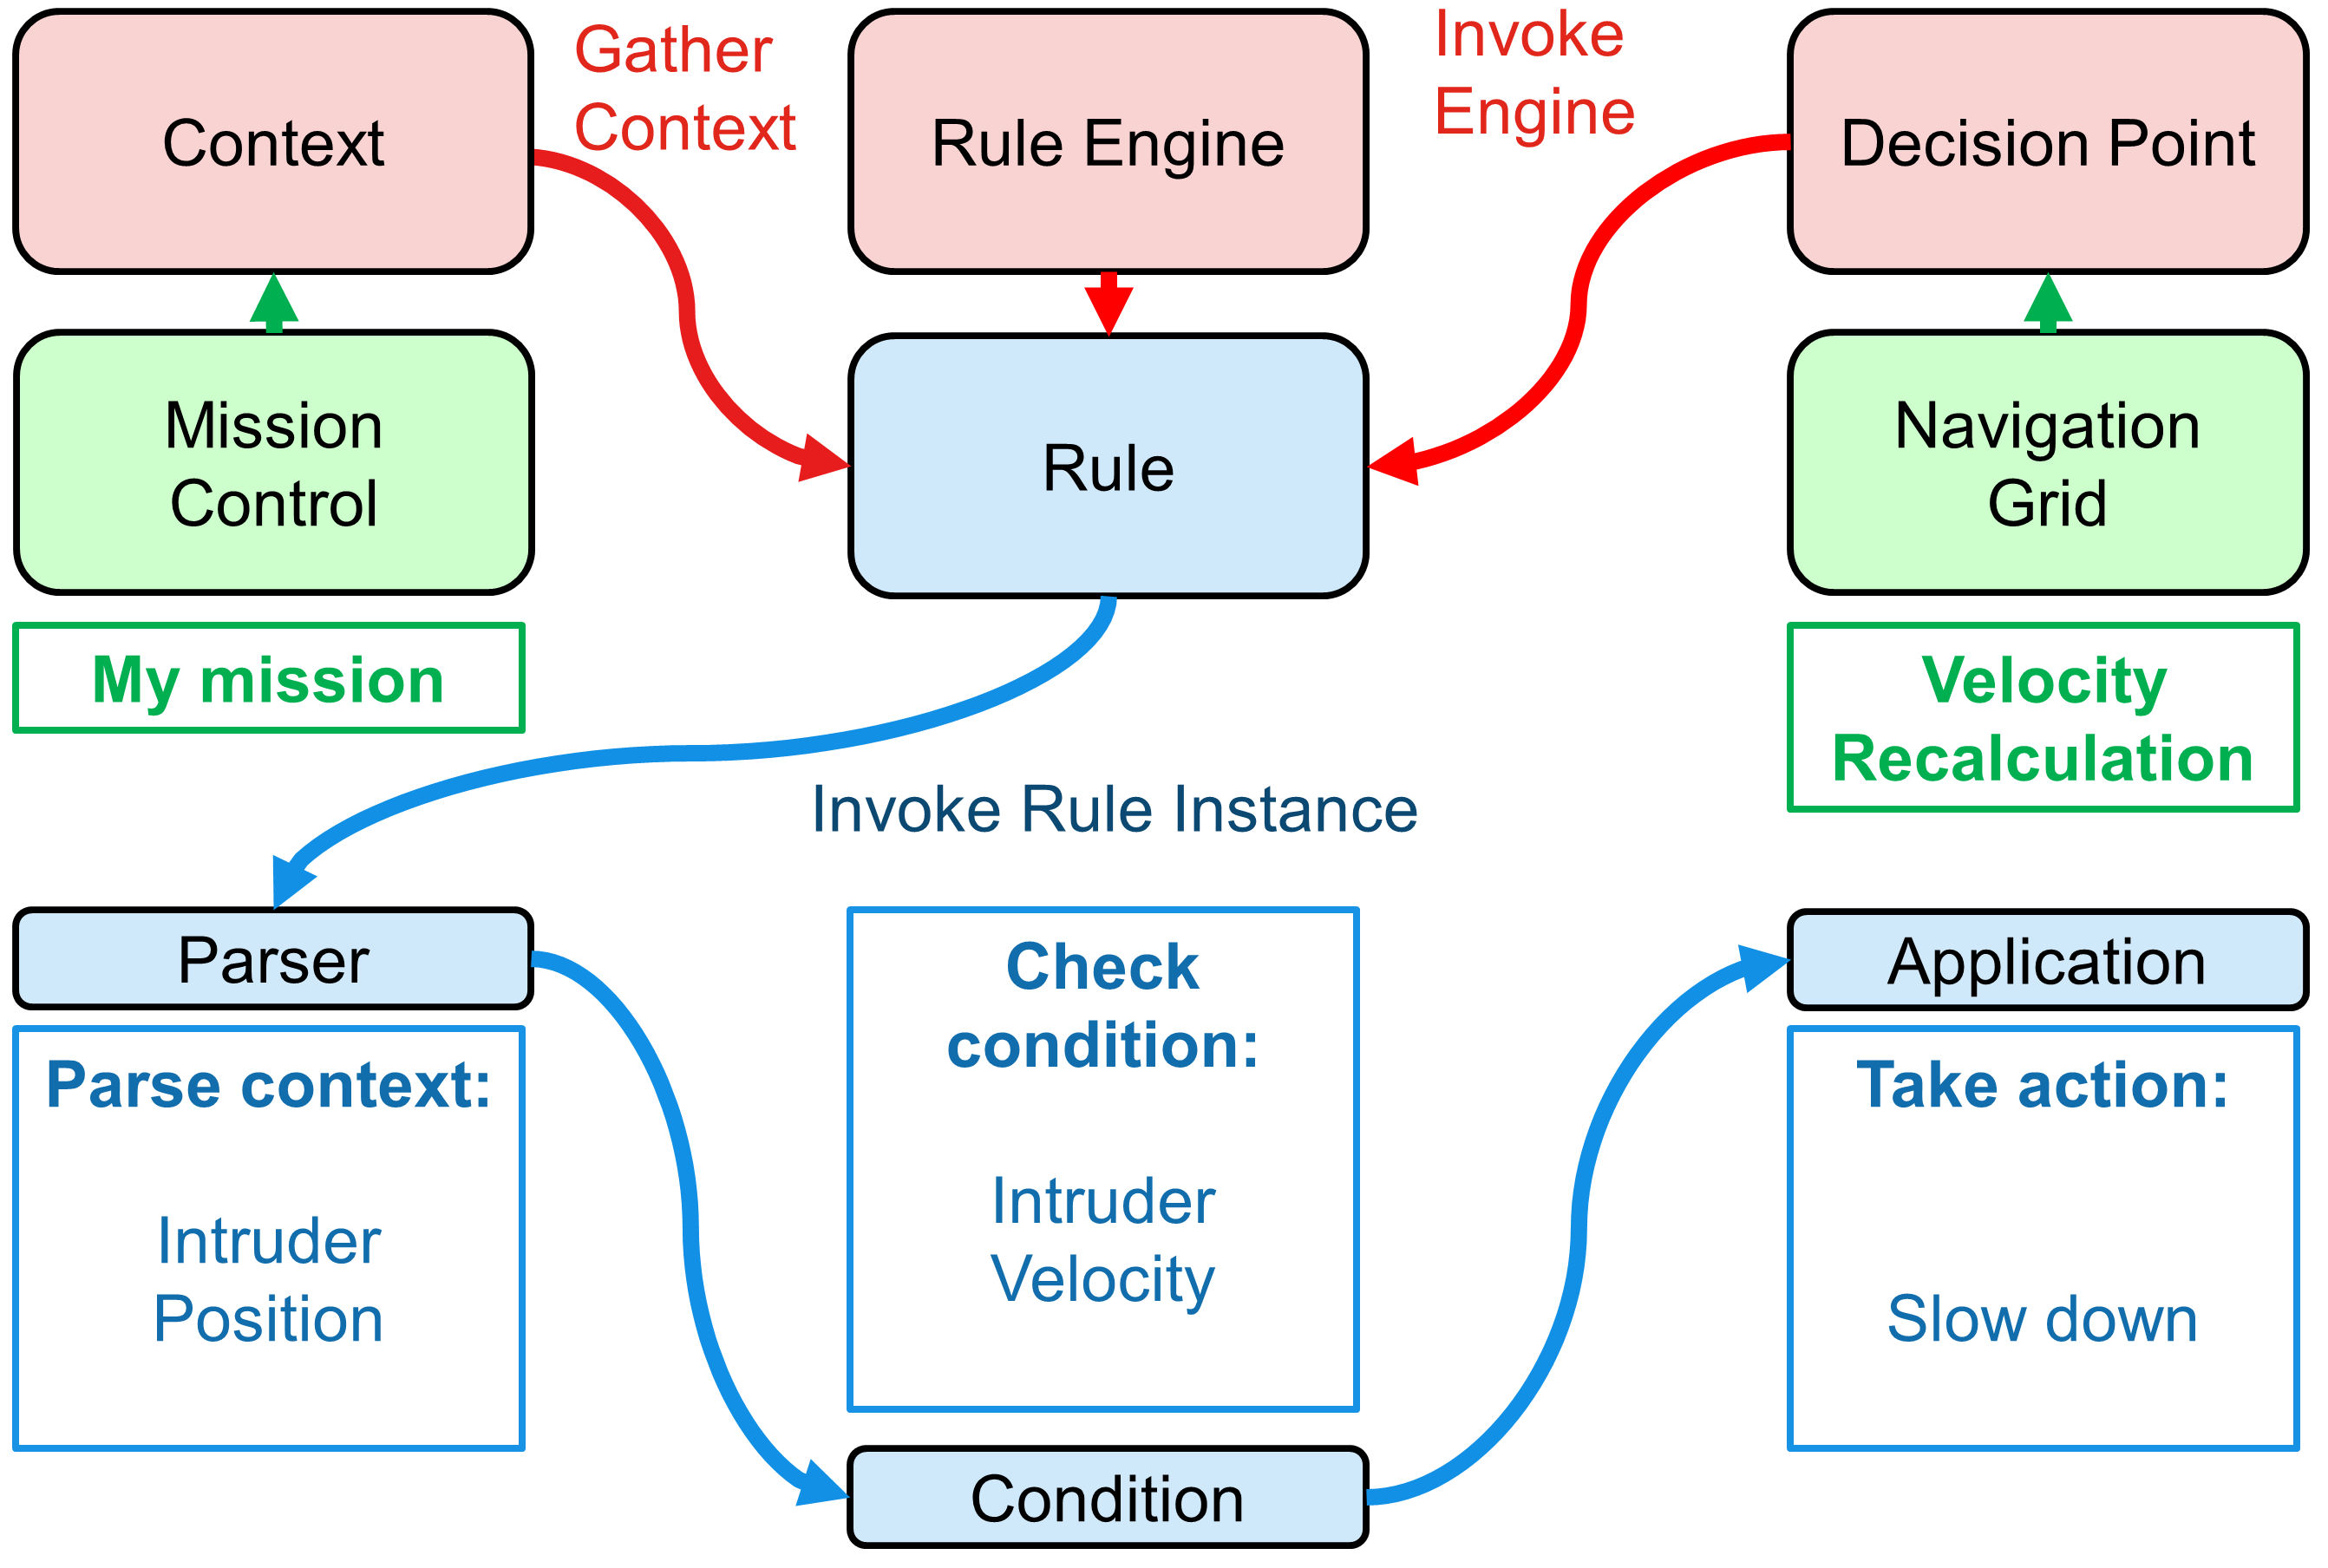
\includegraphics[width=0.7\linewidth]{\FIGDIR/RE013RuleEngineBasicArchitecture}
    \caption{Rule engine components overview.}
    \label{fig:RuleEngineBasicArchitecture}
\end{figure}

\paragraph{Rule Engine:} The program module to inject and run \emph{rules} modifying standard work-flow based on  triggering events. The \emph{aspect-oriented} approach enables to configure rules in \emph{run-time} via predefined process hooks - \emph{Decision Points}. 

\noindent A rules the in context of this work are pieces of code which have a semi-static structure consisting of following parts (fig. \ref{fig:RuleEngineBasicArchitecture}):

\begin{enumerate}
    \item \emph{Decision Point} - hook point in the process where the rule can be attached/detached. If more than one rule is hooked the priority of execution needs to be defined. 
    
    \item \emph{Context} - the \emph{run time context} in a time of \emph{invocation} in our case the \emph{copy} of \emph{Mission Control}, \emph{Avoidance/Navigation Grid} and,  \emph{Collision Cases}.
    
    \item \emph{Parser Method} - optional helper method to parse interesting data set from \emph{Context}. The \emph{parsed data} have better readability.
    
    \item \emph{Condition Check Method} - implementation of the trigger. If the sufficient condition is met, the rule body is applied.
    
    \item \emph{Rule application} - calculations and data structure changes. Mainly, by  \emph{disabling trajectories} in \emph{Reach Set} in our implementation.     
\end{enumerate}

\paragraph{Example:} The \emph{UAS} is flying in controlled airspace.  The \emph{intruder} shows in front of \emph{UAS}. The \emph{UAS} is faster than an \emph{intruder}. The \emph{UAS} tries to obtain permission for \emph{Overtake}. The \emph{UTM} does not allow \emph{overtake}, because of \emph{insufficient UAS maneuverability capability}. The \emph{Rule} (fig. \ref{fig:RuleEngineBasicArchitecture}) with:
\begin{enumerate}
    \item \emph{Context} - UAS Mission Control, containing the actual mission goal and UAS IMU parameters. 
    
    \item \emph{Decision Point} (Joint Point) - Navigation grid, containing projected constraints and reach set approximation.
    
    \item \emph{The rule is invoked:}
    \begin{enumerate}[a.]
        \item \emph{The parser} parses the context which is \emph{intruder`s Position Notification} containing its heading and velocity.
        
        \item \emph{The condition} is checked to \emph{relative intruder velocity}. The \emph{evaluation} is positiv, when the UAS is \emph{pursuing the intruder}.
        
        \item \emph{Application} of \emph{Rule} is the last step, in this case, the \emph{UAS} will slow down.
    \end{enumerate}
\end{enumerate}

\paragraph{Configurability:} The \emph{Rule Engine} enables real-time configuration. The \emph{Enabled Rules Table} have been implemented to enforce specific rules in a specific context. 

The \emph{Rules} can be invoked from \emph{Rule Application}; this enables effective rule chaining and piece-wise functionality split. 

    	\subsection{(R) Rule Implementation}\label{sec:ruleImplementation}

\paragraph{Configuration:} The \emph{Rule Engine Architecture} (fig. \ref{fig:RuleEngineBasicArchitecture}) is configured to handle \emph{UTM functionality} for \emph{Collision Case Resolution} (sec. \ref{sec:collisionCase}).  The overview of \emph{Context} (Green), \emph{Decision Points} (red) and \emph{Rule Invokation} (cyan) is given in (fig. \ref{fig:RuleEngineInstanceLevels}) 

\begin{figure}[H]
    \centering
    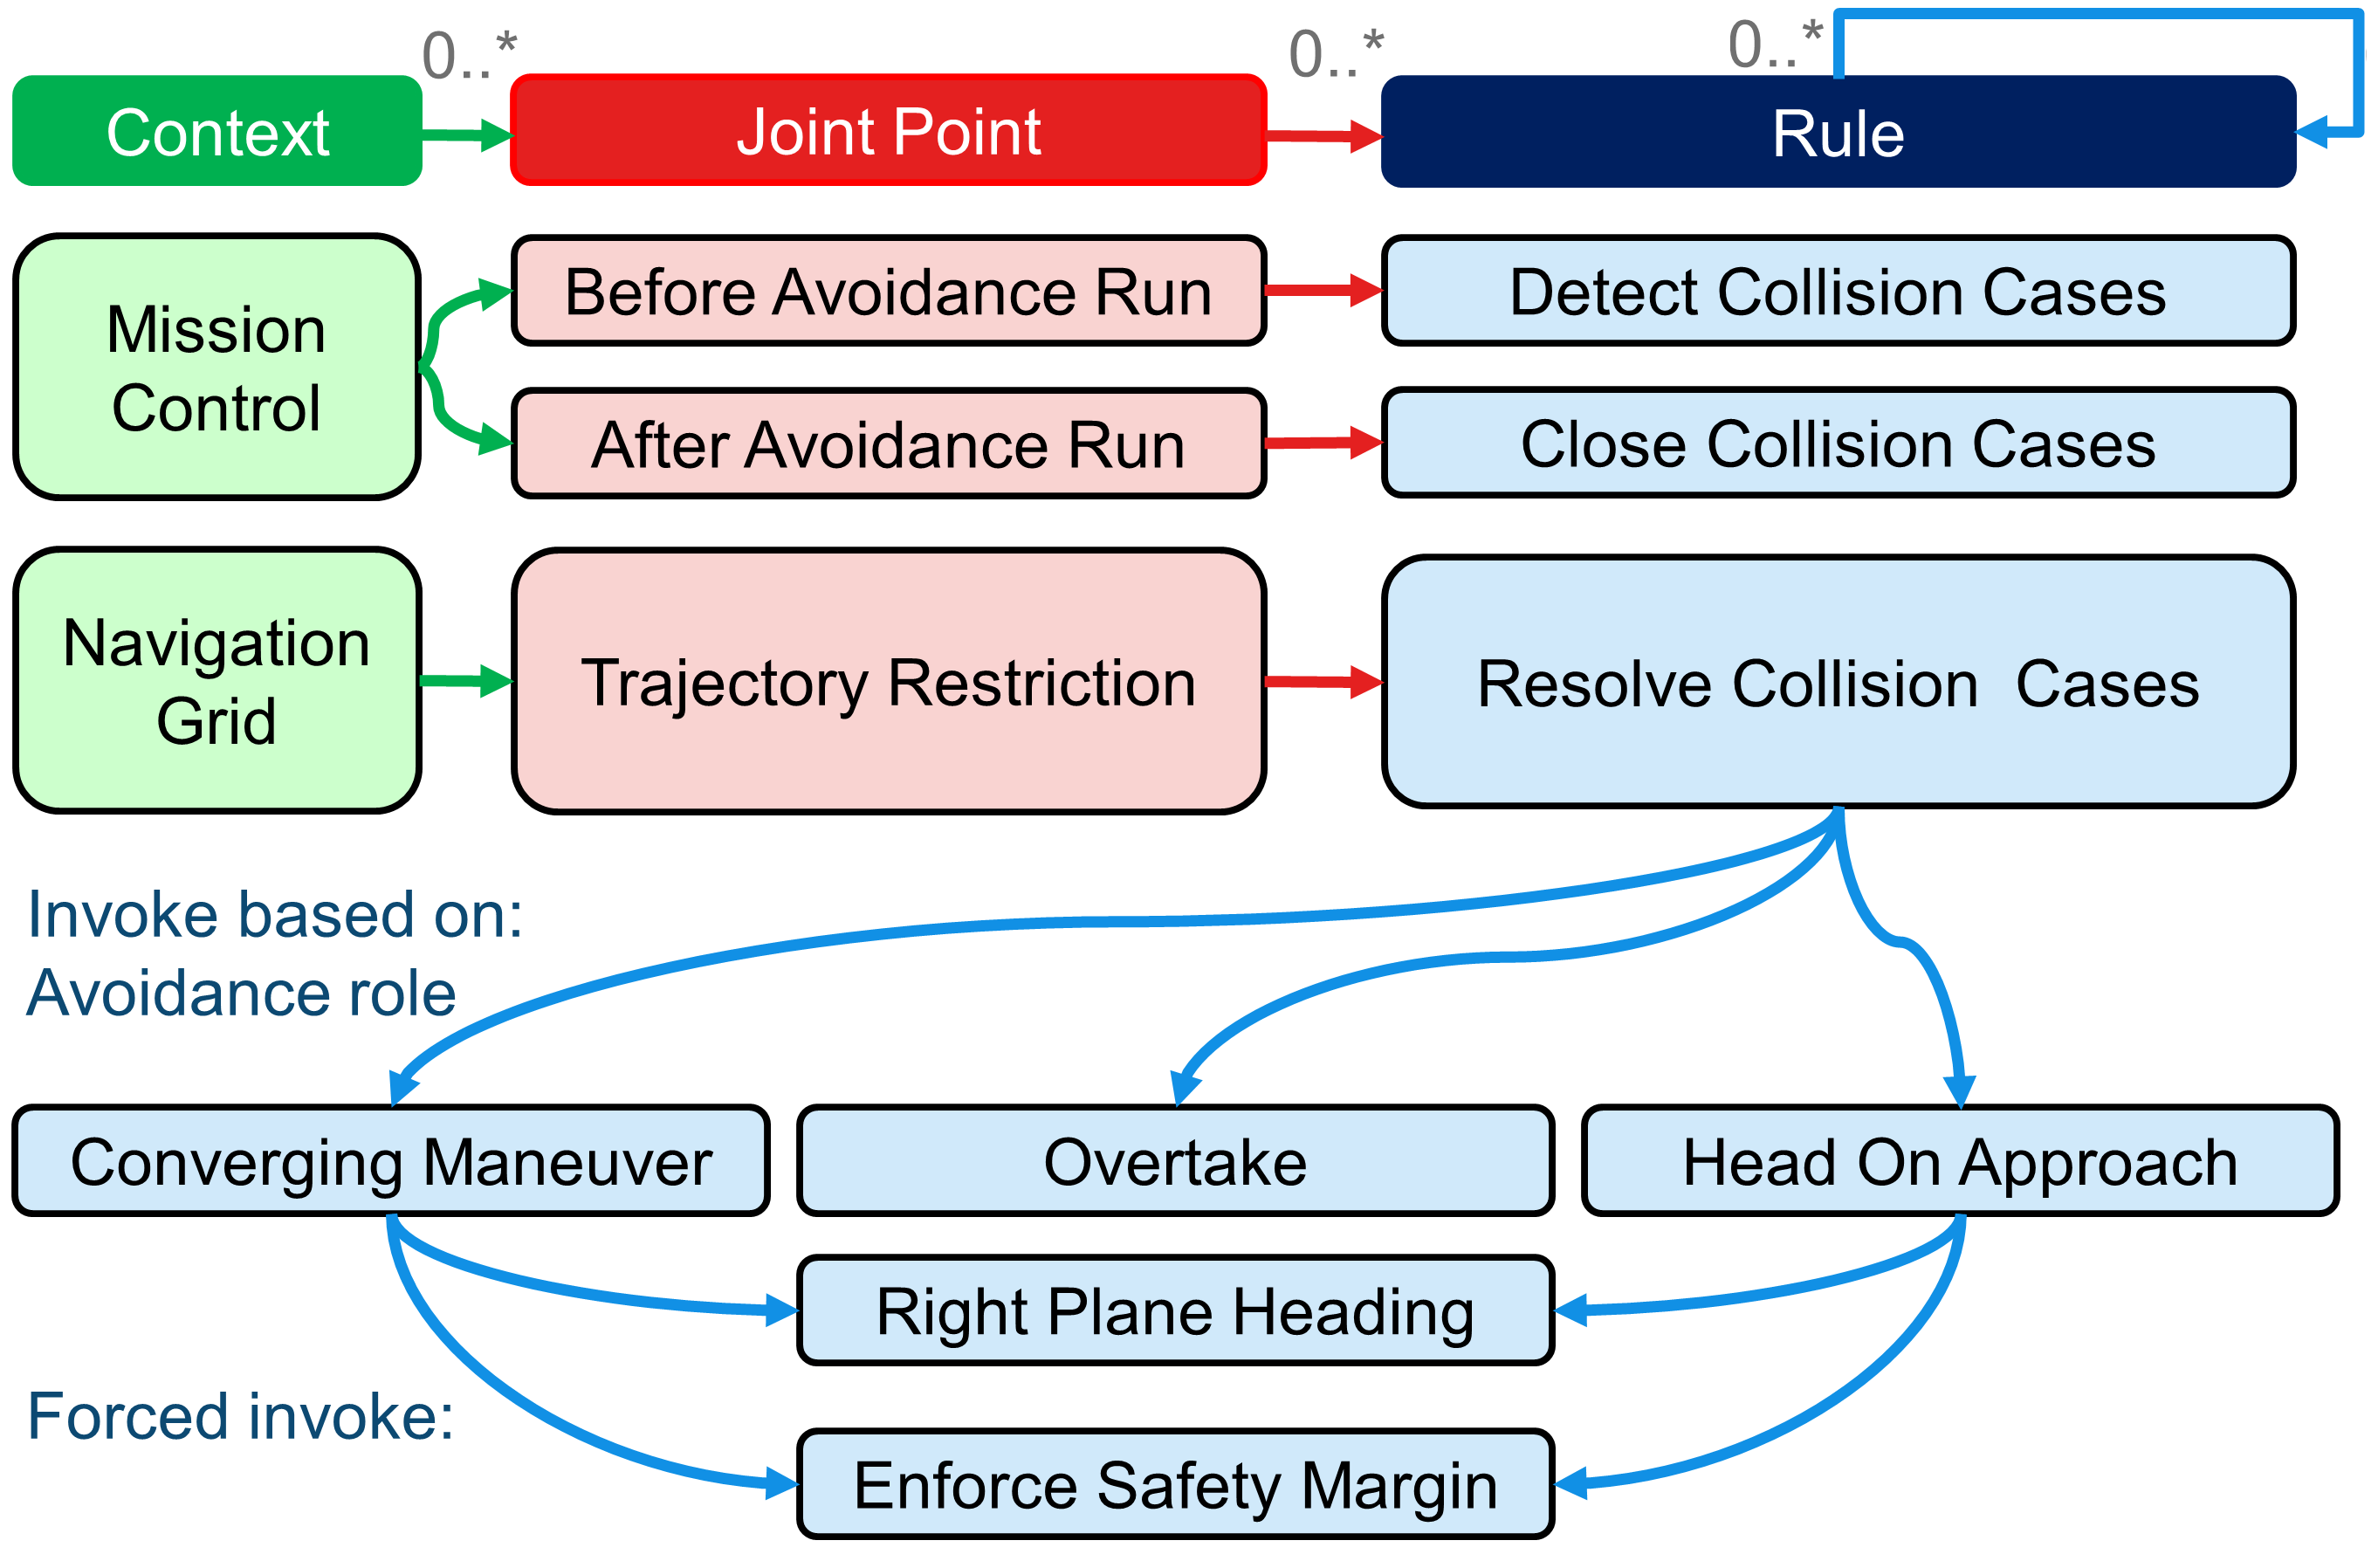
\includegraphics[width=0.7\linewidth]{\FIGDIR/RE014RuleEngineInstanceLevels} 
    \caption{Rule engine initialization with Rules of the air.}
    \label{fig:RuleEngineInstanceLevels}
\end{figure}

\begin{note}
    The \emph{Weather Case} (sec. \ref{sec:weatherCase}) is handled in similar case (fig. \ref{fig:missionControlRunActivityDiagram}) with enforcing \emph{hard constraints} (before step 9.) and \emph{soft constraints} (before step 10.).
\end{note}


\paragraph{Decision Points:} The \emph{Decisions} are bounded to \emph{Mission Control Run Process} (fig. \ref{fig:missionControlRunActivityDiagram}) in following manner:
\begin{enumerate}
    \item \emph{Before Avoidance Run} (before step 7.) - Context: \emph{Mission Control} (Received Collision Cases) - the \emph{UTM} can send some directives it is required to find which are impacting our \emph{UAS}.
    
    \item \emph{Trajectory Restrictions} (after step 7.) - Context: \emph{Navigation Grid} (Trajectory Restrictions) - adaptation of \emph{behaviour} imposed by \emph{active collision cases}.
    
    \item \emph{After Avoidance Run} (after step 11.) - Context: \emph{Mission Control} (Collision Case Resolutions) - our \emph{UAS} will update the status of \emph{Collision Cases} and checks the \emph{avoidance conditions}, then sends the \emph{Resolution Notification} to UAS.
    
\end{enumerate}

\paragraph{Road map:} The \emph{implemented rules}(cyan) are in following categories:
\begin{enumerate}
    \item \emph{Management Rules} - managing collision cases (additional control flow):
        \begin{enumerate}[a.]
            
            \item \emph{Detect Collision Cases} (sec. \ref{sec:detectCollisionCases}) - the detection of active participation in received \emph{collision cases} and generation of \emph{restrictions}.
            
            \item \emph{Resolve Collision Cases} (sec. \ref{sec:ruleResolveCollisionCase}) - the enforcement of \emph{active avoidance roles} in \emph{collision cases}. The one \emph{Restriction Rule} is invoked directly.
            
            \item \emph{Close Collision Cases} (sec. \ref{sec:ruleCloseCollisionCases}) - impact calculation and \emph{Resolution Notification} to \emph{UTM} authority.
        \end{enumerate}
    
    \item \emph{Restriction Rules} - restricting the \emph{Navigation Grid} trajectories or altering \emph{goal waypoint} based on \emph{selected collision cases}:
    \begin{enumerate}[a.]
        \item \emph{Converging Maneuver} (sec. \ref{sec:ruleConvergingManuever}) implementation of \emph{Converging Avoidance} (sec. \ref{sec:handlingConvergingManuever}).
        
        \item \emph{Head On Approach} (sec. \ref{sec:ruleHeadOnApproach}) implementation of \emph{Virtual Roundabout Enforcement} (sec. \ref{sec:handlingHeadOnApproach}).
        
        \item \emph{Overtake} (sec. \ref{sec:ruleOvertake}) implementation of \emph{overtake maneuver} for \emph{Overtaking plane} (sec. \ref{sec:handlingOvertakeManuever}).
    \end{enumerate}
    
    \item \emph{Miscellaneous Rules} - reused pieces of code in \emph{Head On} and \emph{Converging Situations}:
    \begin{enumerate}[a.]
        \item \emph{Right Plane Heading} (sec. \ref{sec:ruleRightPlaneHeading}) - restrict all trajectories heading to space separated by parametric plane in \emph{Avoidance Grid} which are heading or belonging to plane.
        
        \item \emph{Enforce Safety Margin} (sec. \ref{sec:ruleEnforceSafetyMargin}) - restrict all \emph{Trajectories Segments} which are in proximity of \emph{Collision Point} lesser than \emph{Enforced Safety Margin}.
    \end{enumerate}
\end{enumerate}
    	
%% This adds a line for the Bibliography in the Table of Contents.
\addcontentsline{toc}{chapter}{Bibliography}
%% *** Set the bibliography style. ***
%% (change according to your preference/requirements)
%\bibliographystyle{plain}
%% *** Set the bibliography file. ***
%% ("thesis.bib" by default; change as needed)
\bibliography{thesis}

%% *** NOTE ***
%% If you don't use bibliography files, comment out the previous line
%% and use \begin{thebibliography}...\end{thebibliography}.  (In that
%% case, you should probably put the bibliography in a separate file and
%% `\include' or `\input' it here).

\end{document}
